\documentclass[aspectratio=169,10pt]{beamer}

% =============================================================================
% METROPOLIS METRO SIGNALING - LINE G FINAL DEFENSE PRESENTATION
% Engineering Group 7: CentraleSupélec & Prover Technology
% 10-Minute Timed Defense with Dedicated Q&A Backup Slides
% =============================================================================

\usepackage[utf8]{inputenc}
\usepackage[T1]{fontenc}
\usepackage{lmodern}
\usepackage{microtype}
\usepackage{amsmath,amssymb}
\usepackage{booktabs}
\usepackage{tabularx}
\usepackage{tcolorbox}
\tcbuselibrary{skins,breakable}
\usepackage{tikz}
\usetikzlibrary{arrows.meta,positioning,shapes.geometric,fit,calc}
\usepackage{listings}
\usepackage{graphicx}
\usepackage{hyperref}

% -----------------------------------------------------------------------------
% PROVER & CENTRALESUPÉLEC COLOR PALETTE
% -----------------------------------------------------------------------------
\definecolor{ProverNavy}{RGB}{0,43,73}       % Primary brand deep blue #002B49
\definecolor{ProverTeal}{RGB}{0,163,224}     % Accent bright cyan #00A3E0
\definecolor{ProverDarkSlate}{RGB}{26,43,60} % Deep slate
\definecolor{ProverSlate}{RGB}{74,96,122}    % Secondary slate
\definecolor{MetroOrange}{RGB}{217,119,6}    % Metropolis Transport Orange #D97706
\definecolor{AlertRed}{RGB}{186,12,47}       % Warning Accent Red #BA0C2F
\definecolor{SafeGreen}{RGB}{5,150,105}      % Verification Pass Green #059669
\definecolor{CardBg}{RGB}{248,250,252}       % Card background #F8FAFC
\definecolor{CardBorder}{RGB}{226,232,240}   % Card border #E2E8F0
\definecolor{DarkText}{RGB}{30,41,59}        % Body text #1E293B
\definecolor{MutedGray}{RGB}{100,116,139}    % Muted text #64748B
\definecolor{CodeBg}{RGB}{241,245,249}       % Code background #F1F5F9

% -----------------------------------------------------------------------------
% BEAMER THEME & LAYOUT CONFIGURATION
% -----------------------------------------------------------------------------
\setbeamercolor{normal text}{fg=DarkText,bg=white}
\setbeamercolor{structure}{fg=ProverNavy}
\setbeamercolor{frametitle}{fg=ProverNavy,bg=white}
\setbeamercolor{title}{fg=ProverNavy}
\setbeamercolor{subtitle}{fg=ProverTeal}
\setbeamercolor{author}{fg=DarkText}
\setbeamercolor{date}{fg=ProverSlate}

\hypersetup{
  colorlinks=true,
  linkcolor=ProverNavy,
  urlcolor=ProverTeal,
  citecolor=ProverTeal
}

\setbeamersize{text margin left=8mm,text margin right=8mm}
\setbeamertemplate{navigation symbols}{}
\setbeamertemplate{itemize items}[circle]
\setbeamertemplate{enumerate items}[default]

\pdfstringdefDisableCommands{\def\translate#1{#1}}

% Clean frametitle with Prover Logo on right and tight teal rule
\setbeamerfont{frametitle}{series=\bfseries,size=\fontsize{11}{12.5}}
\setbeamerfont{framesubtitle}{size=\fontsize{7}{8.2}}

\setbeamertemplate{frametitle}{%
  \nointerlineskip%
  \vspace*{1.5mm}%
  \parbox[t]{\textwidth}{%
    \begin{minipage}[c]{0.73\textwidth}%
      {\usebeamerfont{frametitle}\usebeamercolor[fg]{frametitle}\insertframetitle\par}%
      \ifx\insertframesubtitle\@empty\else%
        \vspace*{0.5mm}%
        {\usebeamerfont{framesubtitle}\usebeamercolor[fg]{framesubtitle}\insertframesubtitle\par}%
      \fi%
    \end{minipage}\hfill%
    \begin{minipage}[c]{0.25\textwidth}%
      \raggedleft%
      
\includegraphics[width=\linewidth,height=0.32cm,keepaspectratio]{../logo/LogoProver.pdf}%
    \end{minipage}\par%
    \vspace*{1mm}%
    {\color{ProverTeal}\hrule height 0.6pt}%
  }%
  \vspace*{1mm}%
}

% Clean, well-spaced footline matching slide margins exactly
\setbeamertemplate{footline}{%
  \begin{beamercolorbox}[wd=\paperwidth,ht=3.2mm,dp=2.2mm,leftskip=8mm,rightskip=8mm]{footline}%
    \fontsize{6.5}{7.8}\selectfont\color{ProverSlate}%
    CentraleSupélec $\cdot$ Prover 2026%
    \hfill%
    \color{ProverNavy}\textbf{Line G Interlocking $\cdot$ Engineering Group 7}%
    \hfill%
    \color{ProverSlate}\insertframenumber{} / 22%
  \end{beamercolorbox}%
}

% -----------------------------------------------------------------------------
% LISTINGS SPECIFICATION FOR PISPEC
% -----------------------------------------------------------------------------
\lstdefinelanguage{PiSPEC}{
  keywords={class,inherit,Functions,Equations,Timers,Prove,TestCase,expect,within,during,wait,foreach,true,false,ALL,SOME,PRE},
  keywordstyle=\color{ProverNavy}\bfseries,
  ndkeywords={SELF,ReleaseRequested,RouteRequested,Locked,Clear,CommandedProceed,DetectedNormal,DetectedReverse,LineInput,LineOutput,Holding},
  ndkeywordstyle=\color{ProverTeal}\bfseries,
  sensitive=true,
  comment=[l]{//},
  morecomment=[s]{/*}{*/},
  morecomment=[s]{"""}{"""},
  commentstyle=\color{ProverSlate}\itshape,
  stringstyle=\color{MetroOrange},
  basicstyle=\fontsize{6.2}{7.4}\ttfamily,
  breaklines=true,
  tabsize=2,
  showstringspaces=false
}

% -----------------------------------------------------------------------------
% TCOLORBOX CARD DEFINITIONS
% -----------------------------------------------------------------------------
\newtcolorbox{proverbox}[2][]{
  enhanced,
  colback=CardBg,
  colframe=CardBorder,
  coltitle=ProverNavy,
  fonttitle=\bfseries\fontsize{7.5}{8.8}\selectfont\raggedright,
  title={#2},
  arc=1.2mm,
  boxrule=0.5pt,
  valign=center,
  left=1.5mm,right=1.5mm,top=1.2mm,bottom=1.2mm,
  toptitle=0.6mm,bottomtitle=0.6mm,
  #1
}

\newtcolorbox{alertbox}[2][]{
  enhanced,
  colback=AlertRed!5,
  colframe=AlertRed!40,
  coltitle=AlertRed,
  fonttitle=\bfseries\fontsize{7.5}{8.8}\selectfont,
  title={#2},
  arc=1.2mm,
  boxrule=0.5pt,
  valign=center,
  left=1.5mm,right=1.5mm,top=1.2mm,bottom=1.2mm,
  toptitle=0.6mm,bottomtitle=0.6mm,
  #1
}

\newtcolorbox{safebox}[2][]{
  enhanced,
  colback=SafeGreen!5,
  colframe=SafeGreen!40,
  coltitle=SafeGreen,
  fonttitle=\bfseries\fontsize{7.5}{8.8}\selectfont,
  title={#2},
  arc=1.2mm,
  boxrule=0.5pt,
  valign=center,
  left=1.5mm,right=1.5mm,top=1.2mm,bottom=1.2mm,
  toptitle=0.6mm,bottomtitle=0.6mm,
  #1
}

% -----------------------------------------------------------------------------
% AGENDA TRANSITION SLIDE MACRO WITH HYPERLINKS
% #1 = 0: Overview (all active and clickable)
% #1 = 1 to 5: Section #1 active, others dimmed
% -----------------------------------------------------------------------------
\newcommand{\agendaslide}[1]{%
  \begin{frame}{Table of Contents}{Presentation Structure}
    \vspace*{1.2mm}
    \begin{tikzpicture}[every node/.style={text width=0.94\textwidth, rounded corners=1.5mm, inner sep=3.8pt, align=left}]
      % Item 1
      \ifnum#1=1
        \node[fill=ProverNavy, draw=ProverTeal, line width=0.8pt, text=white] (s1) {
          \hyperlink{sec_topology}{%
            \fontsize{7.8}{9.2}\selectfont \textbf{\color{white}1. Network Topology and Station Modeling} \\[1pt]
            \fontsize{6.5}{7.6}\selectfont\color{white!90} Line G operational corridor, station layouts, SDA methodology and G-ABR modeling%
          }
        };
      \else
        \ifnum#1=0
          \node[fill=CardBg, draw=ProverTeal!60, line width=0.6pt] (s1) {
            \hyperlink{sec_topology}{%
              \fontsize{7.8}{9.2}\selectfont \textbf{\color{ProverNavy}1. Network Topology and Station Modeling} \\[1pt]
              \fontsize{6.5}{7.6}\selectfont\color{DarkText} Line G operational corridor, station layouts, SDA methodology and G-ABR modeling%
            }
          };
        \else
          \node[fill=CardBg!50, draw=CardBorder!50, line width=0.4pt] (s1) {
            \hyperlink{sec_topology}{%
              \fontsize{7.8}{9.2}\selectfont \textbf{\color{MutedGray!60}1. Network Topology and Station Modeling} \\[1pt]
              \fontsize{6.5}{7.6}\selectfont\color{MutedGray!45} Line G operational corridor, station layouts, SDA methodology and G-ABR modeling%
            }
          };
        \fi
      \fi

      % Item 2
      \ifnum#1=2
        \node[fill=ProverNavy, draw=ProverTeal, line width=0.8pt, text=white, below=2mm of s1] (s2) {
          \hyperlink{sec_design}{%
            \fontsize{7.8}{9.2}\selectfont \textbf{\color{white}2. Generic Application Design and Testing} \\[1pt]
            \fontsize{6.5}{7.6}\selectfont\color{white!90} Safe manual route release logic, inter-station line block protocol and GTS test cases%
          }
        };
      \else
        \ifnum#1=0
          \node[fill=CardBg, draw=ProverTeal!60, line width=0.6pt, below=2mm of s1] (s2) {
            \hyperlink{sec_design}{%
              \fontsize{7.8}{9.2}\selectfont \textbf{\color{ProverNavy}2. Generic Application Design and Testing} \\[1pt]
              \fontsize{6.5}{7.6}\selectfont\color{DarkText} Safe manual route release logic, inter-station line block protocol and GTS test cases%
            }
          };
        \else
          \node[fill=CardBg!50, draw=CardBorder!50, line width=0.4pt, below=2mm of s1] (s2) {
            \hyperlink{sec_design}{%
              \fontsize{7.8}{9.2}\selectfont \textbf{\color{MutedGray!60}2. Generic Application Design and Testing} \\[1pt]
              \fontsize{6.5}{7.6}\selectfont\color{MutedGray!45} Safe manual route release logic, inter-station line block protocol and GTS test cases%
            }
          };
        \fi
      \fi

      % Item 3
      \ifnum#1=3
        \node[fill=ProverNavy, draw=ProverTeal, line width=0.8pt, text=white, below=2mm of s2] (s3) {
          \hyperlink{sec_verification}{%
            \fontsize{7.8}{9.2}\selectfont \textbf{\color{white}3. Formal Safety Specification and Verification} \\[1pt]
            \fontsize{6.5}{7.6}\selectfont\color{white!90} 12 CENELEC EN 50128 invariant properties, PiSPEC refinements and inductive proof insights%
          }
        };
      \else
        \ifnum#1=0
          \node[fill=CardBg, draw=ProverTeal!60, line width=0.6pt, below=2mm of s2] (s3) {
            \hyperlink{sec_verification}{%
              \fontsize{7.8}{9.2}\selectfont \textbf{\color{ProverNavy}3. Formal Safety Specification and Verification} \\[1pt]
              \fontsize{6.5}{7.6}\selectfont\color{DarkText} 12 CENELEC EN 50128 invariant properties, PiSPEC refinements and inductive proof insights%
            }
          };
        \else
          \node[fill=CardBg!50, draw=CardBorder!50, line width=0.4pt, below=2mm of s2] (s3) {
            \hyperlink{sec_verification}{%
              \fontsize{7.8}{9.2}\selectfont \textbf{\color{MutedGray!60}3. Formal Safety Specification and Verification} \\[1pt]
              \fontsize{6.5}{7.6}\selectfont\color{MutedGray!45} 12 CENELEC EN 50128 invariant properties, PiSPEC refinements and inductive proof insights%
            }
          };
        \fi
      \fi

      % Item 4
      \ifnum#1=4
        \node[fill=ProverNavy, draw=ProverTeal, line width=0.8pt, text=white, below=2mm of s3] (s4) {
          \hyperlink{sec_simulation}{%
            \fontsize{7.8}{9.2}\selectfont \textbf{\color{white}4. Distributed Simulation and Demonstration} \\[1pt]
            \fontsize{6.5}{7.6}\selectfont\color{white!90} Multi-station MQTT architecture and full-line train traversal screen recording%
          }
        };
      \else
        \ifnum#1=0
          \node[fill=CardBg, draw=ProverTeal!60, line width=0.6pt, below=2mm of s3] (s4) {
            \hyperlink{sec_simulation}{%
              \fontsize{7.8}{9.2}\selectfont \textbf{\color{ProverNavy}4. Distributed Simulation and Demonstration} \\[1pt]
              \fontsize{6.5}{7.6}\selectfont\color{DarkText} Multi-station MQTT architecture and full-line train traversal screen recording%
            }
          };
        \else
          \node[fill=CardBg!50, draw=CardBorder!50, line width=0.4pt, below=2mm of s3] (s4) {
            \hyperlink{sec_simulation}{%
              \fontsize{7.8}{9.2}\selectfont \textbf{\color{MutedGray!60}4. Distributed Simulation and Demonstration} \\[1pt]
              \fontsize{6.5}{7.6}\selectfont\color{MutedGray!45} Multi-station MQTT architecture and full-line train traversal screen recording%
            }
          };
        \fi
      \fi

      % Item 5
      \ifnum#1=5
        \node[fill=ProverNavy, draw=ProverTeal, line width=0.8pt, text=white, below=2mm of s4] (s5) {
          \hyperlink{sec_problems}{%
            \fontsize{7.8}{9.2}\selectfont \textbf{\color{white}5. Problems Encountered and Project Conclusion} \\[1pt]
            \fontsize{6.5}{7.6}\selectfont\color{white!90} Baseline GA logic defects, clock cycle anomalies, race condition solutions and conclusions%
          }
        };
      \else
        \ifnum#1=0
          \node[fill=CardBg, draw=ProverTeal!60, line width=0.6pt, below=2mm of s4] (s5) {
            \hyperlink{sec_problems}{%
              \fontsize{7.8}{9.2}\selectfont \textbf{\color{ProverNavy}5. Problems Encountered and Project Conclusion} \\[1pt]
              \fontsize{6.5}{7.6}\selectfont\color{DarkText} Baseline GA logic defects, clock cycle anomalies, race condition solutions and conclusions%
            }
          };
        \else
          \node[fill=CardBg!50, draw=CardBorder!50, line width=0.4pt, below=2mm of s4] (s5) {
            \hyperlink{sec_problems}{%
              \fontsize{7.8}{9.2}\selectfont \textbf{\color{MutedGray!60}5. Problems Encountered and Project Conclusion} \\[1pt]
              \fontsize{6.5}{7.6}\selectfont\color{MutedGray!45} Baseline GA logic defects, clock cycle anomalies, race condition solutions and conclusions%
            }
          };
        \fi
      \fi
    \end{tikzpicture}
  \end{frame}
}

% =============================================================================
% PRESENTATION SLIDES
% =============================================================================
\begin{document}

% -----------------------------------------------------------------------------
% SLIDE 1: TITLE SLIDE (Mirrors report.tex Cover Page)
% -----------------------------------------------------------------------------
{
\setbeamertemplate{footline}{}
\begin{frame}[plain]
  \vspace*{2mm}
  \noindent
  \begin{minipage}[c]{0.45\textwidth}
    
\includegraphics[height=1.1cm,keepaspectratio]{../logo/LogoCS.pdf}
  \end{minipage}%
  \hfill
  \begin{minipage}[c]{0.45\textwidth}
    \raggedleft
    
\includegraphics[height=0.45cm,keepaspectratio]{../logo/LogoProver.pdf}
  \end{minipage}

  \vspace{3.5mm}
  {\Large\bfseries\color{ProverNavy} CentraleSupélec\par}
  \vspace{0.8mm}
  {\fontsize{8}{9.5}\selectfont\bfseries\color{ProverSlate} Engineering Integration Project (EI) - In Partnership with Prover Technology\par}

  \vspace{4.5mm}
  {\fontsize{14}{17}\selectfont\bfseries\color{ProverNavy} Modernization of the Metropolis Metro Signaling Network\par}
  \vspace{1.5mm}
  {\fontsize{8.5}{11}\selectfont\bfseries\color{ProverTeal} Engineering Design, Formal Safety Verification and Interactive Simulation for Line G\par}
  \vspace{1.2mm}
  {\fontsize{8.5}{10.5}\selectfont\bfseries\color{MetroOrange} Engineering Group 7\par}

  \vspace{4mm}
  {\fontsize{8}{9.5}\selectfont\bfseries\color{ProverNavy} Engineering Project Team:\par}
  \vspace{1.5mm}
  \begin{minipage}{\textwidth}
    \centering\fontsize{7.5}{9.2}\selectfont\bfseries\color{DarkText}
    \begin{tabular}{cc}
      Gabriel da Costa & Tiago dos Santos Closs \\[2pt]
      Pedro Lubaszewski Lima & Sebastián Pari Medina
    \end{tabular}
  \end{minipage}

  \vfill
  \centering
  {\fontsize{7}{8.5}\selectfont\color{MutedGray} CentraleSupélec, Gif-sur-Yvette\par}
  \vspace{0.6mm}
  {\fontsize{7}{8.5}\selectfont\color{MutedGray} November 6, 2026\par}
  \vspace*{1mm}
\end{frame}
}

% -----------------------------------------------------------------------------
% SLIDE 2: PRESENTATION CONTENTS OVERVIEW (Clickable)
% -----------------------------------------------------------------------------
\agendaslide{0}

% =============================================================================
% SECTION 1: NETWORK TOPOLOGY AND STATION MODELING
% =============================================================================
\agendaslide{1}

% -----------------------------------------------------------------------------
% SLIDE 3: LINE G TOPOLOGY & OPERATIONAL CONTEXT
% -----------------------------------------------------------------------------
\begin{frame}[label=sec_topology]{Line G Network Topology}{Modernization of five interlocking stations under SIL 4 standards}
  \begin{columns}[c]
    \begin{column}{0.48\textwidth}
      \begin{proverbox}{Industrial Scope and Network Context}
        \begin{itemize}\setlength{\itemsep}{0.8pt}\fontsize{6.8}{8}\selectfont
          \item Modernization of Metropolis Line G connecting the western exhibition park to the eastern tech hub.
          \item Zero route collision, continuous flank protection and strict switch correspondence before clearing signals.
          \item \textbf{Key Assets Across Line G:}
            \begin{itemize}\fontsize{6.2}{7.4}\selectfont
              \item \textbf{5} Interlocking Stations (SAs)
              \item \textbf{26} Point Machines (Switches)
              \item \textbf{90} Light Signals (Routes, Shunts and Exits)
              \item \textbf{16} Platform and Siding Tracks
            \end{itemize}
        \end{itemize}
      \end{proverbox}
      \vspace{-2mm}
      \begin{safebox}{Line Key Performance Indicator}
        \centering\fontsize{6.8}{8}\selectfont
        \textbf{100\% Safety Property Proof} across all five stations without deadlocks.
      \end{safebox}
    \end{column}

    \begin{column}{0.50\textwidth}
      \begin{proverbox}{Station Breakdown: West to East (Line G)}
        \fontsize{6.5}{7.6}\selectfont
        \begin{tabularx}{\linewidth}{lXcc}
          \toprule
          \textbf{Station} & \textbf{Typology} & \textbf{Sw.} & \textbf{Sig.} \\
          \midrule
          \textbf{G-PEX} & Terminus (5 platforms) & 5 & 15 \\
          \textbf{G-EME} & Double Crossover + Line H & 5 & 18 \\
          \textbf{G-ABR} & Loop station + 2 sidings & 6 & 20 \\
          \textbf{G-CLA} & Scissors Crossover + Line D & 5 & 15 \\
          \textbf{G-TEC} & Fan Terminus (5 platforms) & 5 & 22 \\
          \bottomrule
        \end{tabularx}
      \end{proverbox}

      \vspace{0.8mm}
      \centering
      
\begin{tikzpicture}[scale=0.82, every node/.style={transform shape}]
        \node[draw=ProverNavy, fill=CardBg, rounded corners, inner sep=2.5pt, font=\fontsize{6.5}{7.5}\selectfont\bfseries] (pex) {G-PEX};
        \node[draw=ProverNavy, fill=CardBg, rounded corners, inner sep=2.5pt, font=\fontsize{6.5}{7.5}\selectfont\bfseries, right=6mm of pex] (eme) {G-EME};
        \node[draw=ProverNavy, fill=ProverNavy, text=white, rounded corners, inner sep=2.5pt, font=\fontsize{6.5}{7.5}\selectfont\bfseries, right=6mm of eme] (abr) {G-ABR};
        \node[draw=ProverNavy, fill=CardBg, rounded corners, inner sep=2.5pt, font=\fontsize{6.5}{7.5}\selectfont\bfseries, right=6mm of abr] (cla) {G-CLA};
        \node[draw=ProverNavy, fill=CardBg, rounded corners, inner sep=2.5pt, font=\fontsize{6.5}{7.5}\selectfont\bfseries, right=6mm of cla] (tec) {G-TEC};

        \draw[<->, thick, ProverTeal] (pex) -- node[above, font=\fontsize{5}{6}\selectfont] {VG1/2} (eme);
        \draw[<->, thick, ProverTeal] (eme) -- node[above, font=\fontsize{5}{6}\selectfont] {VG1/2} (abr);
        \draw[<->, thick, ProverTeal] (abr) -- node[above, font=\fontsize{5}{6}\selectfont] {VG1/2} (cla);
        \draw[<->, thick, ProverTeal] (cla) -- node[above, font=\fontsize{5}{6}\selectfont] {VG1/2} (tec);
      \end{tikzpicture}\par
    \end{column}
  \end{columns}
\end{frame}

% -----------------------------------------------------------------------------
% SLIDE 4: SDA METHODOLOGY & STATION MODELING
% -----------------------------------------------------------------------------
\begin{frame}{Signaling Design Automation (SDA)}{Decoupling generic interlocking rules from specific station layouts}
  \begin{columns}[c]
    \begin{column}{0.48\textwidth}
      \begin{proverbox}{The SDA Formal Paradigm}
        \begin{itemize}\setlength{\itemsep}{1.2pt}\fontsize{6.8}{8}\selectfont
          \item \textbf{Generic Application (GA):}
            Reusable signaling logic written in PiSPEC:
            \begin{itemize}\fontsize{6.2}{7.4}\selectfont
              \item \textbf{OM}: Abstract topological object definitions
              \item \textbf{GDS}: Dynamic equations and safety timers
              \item \textbf{GSS}: Formal safety invariants to prove
              \item \textbf{GTS}: Behavioral simulation test suite
            \end{itemize}
          \item \textbf{Specific Application (SA):}
            Instantiated automatically from station track plans (\texttt{.isy}):
            \begin{itemize}\fontsize{6.2}{7.4}\selectfont
              \item Zero custom code written per station
              \item Guaranteed portability and consistency
            \end{itemize}
        \end{itemize}
      \end{proverbox}
    \end{column}

    \begin{column}{0.50\textwidth}
      \begin{proverbox}{G-ABR (Abrial) Topological Modeling}
        \begin{itemize}\setlength{\itemsep}{1.2pt}\fontsize{6.8}{8}\selectfont
          \item Modeled the most complex intermediate station on Line G:
            \begin{itemize}\fontsize{6.2}{7.4}\selectfont
              \item Main through tracks \texttt{T23} and \texttt{T24}
              \item Siding spurs \texttt{P9} and \texttt{P10} protected by derailers
              \item 6 switches (\texttt{sw-11} to \texttt{sw-16}) forming double bypass
            \end{itemize}
          \item \textbf{Challenge:} Ensuring non-conflicting shunt movements to sidings \texttt{P9}/\texttt{P10} while mainline expresses traverse through \texttt{P7}/\texttt{P8}.
        \end{itemize}
      \end{proverbox}

      \begin{safebox}{Engineering Best Practice}
        \fontsize{6.5}{7.8}\selectfont
        Separation of safety logic (GSS) from implementation (GDS) enabled immediate discovery of design edge cases early in the lifecycle.
      \end{safebox}
    \end{column}
  \end{columns}
\end{frame}

% =============================================================================
% SECTION 2: GENERIC APPLICATION DESIGN AND TESTING
% =============================================================================
\agendaslide{2}

% -----------------------------------------------------------------------------
% SLIDE 5: OM & GDS ADDITIONS: SAFE MANUAL ROUTE RELEASE
% -----------------------------------------------------------------------------
\begin{frame}[fragile,label=sec_design]{Manual Route Release Design}{Safe route cancellation with 30-second delay and overlap protection}
  \begin{columns}[c]
    \begin{column}{0.48\textwidth}
      \begin{proverbox}{The Engineering Challenge (MPS-21 to MPS-26)}
        \begin{itemize}\setlength{\itemsep}{1.2pt}\fontsize{6.8}{8}\selectfont
          \item Dispatchers require canceling locked routes when trains are halted or rerouted.
          \item \textbf{Safety Hazard:} An immediate release could derail an approaching train or move a switch under rolling stock.
          \item \textbf{Engineered Solution in GDS:}
            \begin{itemize}\fontsize{6.2}{7.4}\selectfont
              \item 30-second fixed off-delay countdown (\texttt{ReleaseTimer})
              \item \texttt{Holding} latch to maintain lock on shared sections
              \item Re-requested routes during countdown remain blocked
            \end{itemize}
        \end{itemize}
      \end{proverbox}

      \begin{safebox}{Release Invariant}
        \fontsize{6.5}{7.8}\selectfont
        \textbf{Mutual Exclusion:} If another set route shares a section with the releasing route, the shared section is \emph{never} released prematurely.
      \end{safebox}
    \end{column}

    \begin{column}{0.50\textwidth}
      \begin{proverbox}{PiSPEC Formal Implementation (GDS\_ROUTE.tm)}
\begin{lstlisting}[language=PiSPEC,basicstyle=\fontsize{5.8}{7}\ttfamily]
ReleaseTimer :=
  SELF.ReleaseRequested &
  SOME rts:SELF.route_sections rts.Locked &
  ~SOME rt1 (
    ~(rt1 = SELF) & set(rt1) &
    SOME rts:SELF.route_sections route_sections(rt1, rts)
  ) &
  ~SELF.immediate_manual_release;

Holding :=
  SELF.ready_to_lock #
  SELF.Holding & SOME rts:SELF.route_sections rts.Locked &
  ~SELF.JustUnlocked;

Timers:
  ReleaseTimer (SET=0 SEC, CLEAR=30 SEC, FIXED);
\end{lstlisting}
      \end{proverbox}
    \end{column}
  \end{columns}
\end{frame}

% -----------------------------------------------------------------------------
% SLIDE 6: LINE BLOCK INTERFACE & HANDSHAKE
% -----------------------------------------------------------------------------
\begin{frame}{Line Block Interface and Exit Signals}{Boundary handshake protocol protecting inter-station tracks}
  \begin{columns}[c]
    \begin{column}{0.50\textwidth}
      \begin{proverbox}{Line Block Boundary Handshake Logic}
        \begin{itemize}\setlength{\itemsep}{1.2pt}\fontsize{6.8}{8}\selectfont
          \item Stations coordinate across boundary tracks (\texttt{VG1}, \texttt{VG2}) using bidirectional interface variables:
            \begin{itemize}\fontsize{6.2}{7.4}\selectfont
              \item \texttt{LineOutput}: Transmitted to neighbor when block is free
              \item \texttt{LineInput}: Received from neighbor authorizing dispatch
            \end{itemize}
          \item \textbf{Safety Conditioning in Exit Signals:}
            \begin{itemize}\fontsize{6.2}{7.4}\selectfont
              \item Exit signal clears to green \emph{if and only if}:
                \begin{itemize}\fontsize{6}{7}\selectfont
                  \item Route end-locking is established
                  \item \texttt{LineInput} is asserted by adjacent station
                  \item Intermediate line track circuit is fully clear
                \end{itemize}
            \end{itemize}
        \end{itemize}
      \end{proverbox}
    \end{column}

    \begin{column}{0.48\textwidth}
      \begin{proverbox}{Exit Signal GDS Equation (\texttt{EXIT\_SIGNAL.tm})}
        \fontsize{6.8}{8}\selectfont
        \begin{equation*}
          \begin{aligned}
            \texttt{LineOutput} := & \sim\texttt{end\_locked(SELF)} \\
            & \land \sim\texttt{CommandedProceed(SELF)} \\
            & \land \texttt{SOME tc:SELF.track\_after} \\
            & \qquad \texttt{tc.Clear}
          \end{aligned}
        \end{equation*}
        \vspace{-2mm}
        \begin{itemize}\setlength{\itemsep}{1pt}\fontsize{6.5}{7.6}\selectfont
          \item Keeps the line track reserved while a train travels between stations, even after departure route sections unlock.
        \end{itemize}
      \end{proverbox}

      \begin{alertbox}{Critical Fix Implemented}
        \fontsize{6.5}{7.6}\selectfont
        Exit signals were decoupled from generic signal protection areas, preventing false clearances on station boundaries.
      \end{alertbox}
    \end{column}
  \end{columns}
\end{frame}

% -----------------------------------------------------------------------------
% SLIDE 7: GTS AUTOMATED TEST SUITE EXECUTION
% -----------------------------------------------------------------------------
\begin{frame}{Automated Dynamic Testing (GTS)}{Behavioral test cases validating timing delays and safety boundaries}
  \begin{columns}[c]
    \begin{column}{0.55\textwidth}
      \begin{proverbox}{Test Suite Coverage Across Line G}
        \fontsize{6.5}{7.8}\selectfont
        \begin{tabularx}{\linewidth}{lXcc}
          \toprule
          \textbf{Test} & \textbf{Focus Description} & \textbf{Time} & \textbf{Result} \\
          \midrule
          \textbf{TC 1} & Standard route setting, locking and release & 45\,s & \textbf{\color{SafeGreen}PASS} \\
          \textbf{TC 2} & Switch throw ($<1\text{s}$ loss, $<4\text{s}$ det), lock & 35\,s & \textbf{\color{SafeGreen}PASS} \\
          \textbf{TC 3} & Line block exit signal and line reservation & 55\,s & \textbf{\color{SafeGreen}PASS} \\
          \textbf{TC 4} & Manual release: 30s delay and multi-section & 60\,s & \textbf{\color{SafeGreen}PASS} \\
          \bottomrule
        \end{tabularx}
      \end{proverbox}
    \end{column}

    \begin{column}{0.43\textwidth}
      \begin{proverbox}{Timing Realism in Test Case 2}
        \begin{itemize}\setlength{\itemsep}{1.5pt}\fontsize{6.5}{7.6}\selectfont
          \item Switch simulated throwing time: \textbf{3.0\,s}.
          \item Expectation window tuned to \textbf{4.0\,s} to prevent false test timeouts while validating real electromechanical behavior.
        \end{itemize}
      \end{proverbox}

      \begin{safebox}{Test Suite Conclusion}
        \centering\fontsize{7}{8.2}\selectfont
        \textbf{100\% Pass Rate} achieved across all five Line G project stations in Prover iLock simulation harness.
      \end{safebox}
    \end{column}
  \end{columns}
\end{frame}

% =============================================================================
% SECTION 3: FORMAL SAFETY SPECIFICATION AND VERIFICATION
% =============================================================================
\agendaslide{3}

% -----------------------------------------------------------------------------
% SLIDE 8: FORMAL SAFETY SPECIFICATION (GSS) STRATEGY
% -----------------------------------------------------------------------------
\begin{frame}[label=sec_verification]{Formal Safety Specification (GSS)}{Mathematical verification using Prover iLock Verifier}
  \begin{columns}[c]
    \begin{column}{0.48\textwidth}
      \begin{proverbox}{Defense-in-Depth Verification Layers}
        \begin{enumerate}\setlength{\itemsep}{1.2pt}\fontsize{6.5}{7.6}\selectfont
          \item \textbf{Layer 1: Signal Authority}
            \begin{itemize}\fontsize{6}{7}\selectfont
              \item \texttt{GSS\_01}: Proceed aspect implies unique, locked route
            \end{itemize}
          \item \textbf{Layer 2: Conflict and Flank Protection}
            \begin{itemize}\fontsize{6}{7}\selectfont
              \item \texttt{GSS\_02}: Shared tracks mutually exclusive
              \item \texttt{GSS\_03}: Switches locked in correspondence
              \item \texttt{GSS\_05}: Flank protection established and stable
            \end{itemize}
          \item \textbf{Layer 3: Track Occupancy and End Protection}
            \begin{itemize}\fontsize{6}{7}\selectfont
              \item \texttt{GSS\_04}: Route tracks vacant before clearance
              \item \texttt{GSS\_06}: Route end protection (buffer / signal / line)
              \item \texttt{GSS\_07}: Locked switches cannot move
            \end{itemize}
          \item \textbf{Layer 4: Release and Inter-Station Safety}
            \begin{itemize}\fontsize{6}{7}\selectfont
              \item \texttt{GSS\_08}--\texttt{GSS\_10}: Sequential train-guided release
              \item \texttt{EXIT\_1}--\texttt{EXIT\_2}: Boundary line block safety
            \end{itemize}
        \end{enumerate}
      \end{proverbox}
    \end{column}

    \begin{column}{0.50\textwidth}
      \begin{proverbox}{Why Formal Verification over Testing?}
        \begin{itemize}\setlength{\itemsep}{1.5pt}\fontsize{6.8}{8}\selectfont
          \item \textbf{Testing} demonstrates the presence of bugs in specific sampled traces.
          \item \textbf{Formal Verification} mathematically proves the absence of hazardous states across the entire state space ($>10^{30}$ states).
          \item Inductive invariant proofs verify that safety holds for all reachable cycles $t \to t+1$.
        \end{itemize}
      \end{proverbox}

      \begin{safebox}{SIL 4 Regulatory Standard}
        \centering\fontsize{7}{8.2}\selectfont
        Complies with \textbf{CENELEC EN 50128} requirements for safety-critical railway interlocking software.
      \end{safebox}
    \end{column}
  \end{columns}
\end{frame}

% -----------------------------------------------------------------------------
% SLIDE 9: MATHEMATICAL REFINEMENTS & CRITICAL REQUIREMENTS
% -----------------------------------------------------------------------------
\begin{frame}{Mathematical Safety Refinements}{Resolving counterexamples in route end protection and release}
  \begin{columns}[c]
    \begin{column}{0.50\textwidth}
      \begin{proverbox}{Route End Protection (\texttt{GSS\_06}, MPS-17)}
        \fontsize{6}{7.2}\selectfont
        Tri-partite disjunction covering all three terminus topologies:
        \begin{align*}
          \texttt{Set}(rt) \implies & \texttt{SOME bs:rt.end\_object true} \quad\text{\color{ProverSlate}(Buffer Stop)} \\
          \# & \texttt{SOME esi:rt.end\_object (esi.LineInput} \\
             & \quad \land \texttt{SOME tc:esi.track\_after tc.Clear)} \quad\text{\color{ProverNavy}(Exit)} \\
          \# & \texttt{SOME si1:rt.end\_object (~EXIT\_SIGNAL(si1)} \\
             & \quad \land (\texttt{CommandedProceed}(si1) \lor \texttt{protective}))
        \end{align*}
        \vspace{-2.5mm}
        \begin{itemize}\setlength{\itemsep}{1pt}\fontsize{6}{7.2}\selectfont
          \item Strict exclusion ($\sim\texttt{EXIT\_SIGNAL}$) guarantees exit signals cannot masquerade as standard signals with protection areas.
        \end{itemize}
      \end{proverbox}
    \end{column}

    \begin{column}{0.48\textwidth}
      \begin{proverbox}{Sequential Release Semantics (\texttt{GSS\_10})}
        \fontsize{6.2}{7.4}\selectfont
        Section release requires previous cycle readiness:
        \begin{equation*}
          \begin{aligned}
            & \texttt{PRE Locked}(rts) \land \sim\texttt{Locked}(rts) \land \sim\texttt{ManualUnlock}(rts) \\
            & \implies \texttt{Clear}(rts.\text{tracks}) \land \mathbf{PRE}\,\texttt{ready\_to\_release}(rts)
          \end{aligned}
        \end{equation*}
        \begin{itemize}\setlength{\itemsep}{1pt}\fontsize{6.2}{7.2}\selectfont
          \item Utilizes the \textbf{\texttt{PRE}} temporal operator.
          \item Exempts manual release countdown expiration while maintaining strict train-occupancy requirements during normal traffic.
        \end{itemize}
      \end{proverbox}

      \begin{safebox}{Formal Rigor}
        \fontsize{6.5}{7.6}\selectfont
        Eliminated all four initial counterexamples reported during the pilot baseline.
      \end{safebox}
    \end{column}
  \end{columns}
\end{frame}

% -----------------------------------------------------------------------------
% SLIDE 10: VERIFICATION THOUGHT PROCESS & ARCHITECTURAL SOUNDNESS
% -----------------------------------------------------------------------------
\begin{frame}{Formal Proof Strategy and Insights}{Mathematical rigor ensuring zero-defect safety across Line G}
  \begin{columns}[c]
    \begin{column}{0.50\textwidth}
      \begin{proverbox}{The Inductive Verification Thought Process}
        \begin{itemize}\setlength{\itemsep}{1.2pt}\fontsize{6.5}{7.6}\selectfont
          \item \textbf{Mathematical Formulation:} Translated human-readable safety principles into non-ambiguous first-order logic formulas with temporal quantifiers.
          \item \textbf{1-Step Induction ($k=1$):}
            \begin{itemize}\fontsize{6}{7}\selectfont
              \item Proved that each invariant holds at initialization ($t = 0$).
              \item Proved that if an invariant holds at cycle $t$, it strictly holds at cycle $t + 1$.
            \end{itemize}
          \item \textbf{Architectural Inductivity:}
            Zero manual auxiliary lemmas were required, proving the intrinsic soundness of our Generic Design Specification.
        \end{itemize}
      \end{proverbox}
    \end{column}

    \begin{column}{0.48\textwidth}
      \begin{safebox}{Exhaustive Proof Results Across All 5 Stations}
        \begin{itemize}\setlength{\itemsep}{1.5pt}\fontsize{6.5}{7.6}\selectfont
          \item \textbf{Total Proof Goals:} 60 / 60 (12 properties $\times$ 5 SAs).
          \item \textbf{Success Rate:} \textbf{100\% PROVED} without counterexamples.
          \item \textbf{Proof Engines:} Automated SAT/SMT k-induction in Prover iLock Verifier.
          \item \textbf{Solver Runtime:} Under 90 seconds total for the entire line.
        \end{itemize}
      \end{safebox}

      \begin{proverbox}{Industrial Certification Readiness}
        \fontsize{6.5}{7.6}\selectfont
        Provides absolute mathematical guarantees against train collision, point motor operation under rolling stock and premature release.
      \end{proverbox}
    \end{column}
  \end{columns}
\end{frame}

% =============================================================================
% SECTION 4: DISTRIBUTED SIMULATION AND DEMONSTRATION
% =============================================================================
\agendaslide{4}

% -----------------------------------------------------------------------------
% SLIDE 11: MULTI-STATION DISTRIBUTED SIMULATION VIA MQTT
% -----------------------------------------------------------------------------
\begin{frame}[label=sec_simulation]{Distributed MQTT Simulation Architecture}{Coupling five autonomous Prover iLock instances in real time}
  \begin{columns}[c]
    \begin{column}{0.44\textwidth}
      \begin{proverbox}{Decentralized Architecture}
        \begin{itemize}\setlength{\itemsep}{1.2pt}\fontsize{6.5}{7.6}\selectfont
          \item \textbf{Process Independence:} Each station runs in an isolated Prover iLock simulation process.
          \item \textbf{Local Message Broker:} Standard broker running on \texttt{localhost:1883}, eliminating cloud network latency.
          \item \textbf{Border Telemetry Synchronization:}
            \begin{itemize}\fontsize{6}{7}\selectfont
              \item Boundary signals: \texttt{SeG1/2-XXX-E/W}
              \item Boundary tracks: \texttt{VG1/2-XXX}
            \end{itemize}
          \item \textbf{Deterministic Exchange:} Sub-millisecond state replication across station boundaries.
        \end{itemize}
      \end{proverbox}

      \vspace*{1.5mm}
      \begin{safebox}{Validation Outcome}
        \fontsize{6.5}{7.6}\selectfont
        Successful train transfer across all four boundary blocks without collision or packet drop.
      \end{safebox}
    \end{column}

    \begin{column}{0.54\textwidth}
      \begin{proverbox}{Distributed Interlocking Architecture}
        \centering\vspace{1mm}
        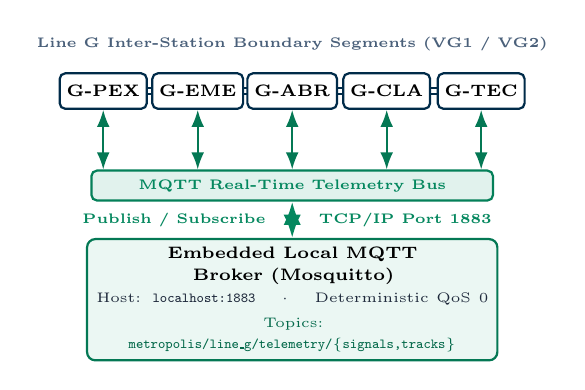
\begin{tikzpicture}[
          x=1cm, y=1cm,
          sta/.style={draw=ProverNavy, fill=white, line width=0.8pt, rounded corners=2pt, font=\fontsize{6}{7.2}\selectfont\bfseries, inner sep=2.5pt, minimum width=0.92cm, minimum height=0.45cm, align=center},
          bus/.style={draw=SafeGreen!85!black, fill=SafeGreen!12, line width=0.8pt, rounded corners=2pt, font=\fontsize{5.2}{6.2}\selectfont\bfseries\color{SafeGreen!90!black}, inner sep=2pt, minimum width=5.1cm, minimum height=0.38cm, align=center},
          broker/.style={draw=SafeGreen!80!black, fill=SafeGreen!8, line width=0.8pt, rounded corners=3pt, font=\fontsize{6.5}{7.8}\selectfont\bfseries, inner sep=3pt, align=center, text width=5.0cm}
        ]
          % Header for rail layer
          \node[font=\fontsize{5.2}{6.2}\selectfont\bfseries\color{ProverSlate}] at (2.8, 3.85) {Line G Inter-Station Boundary Segments (VG1 / VG2)};

          % Double rails behind stations
          \draw[double, double distance=1.4pt, ProverNavy, line width=0.6pt] (0.3, 3.25) -- (5.3, 3.25);

          % 5 Station Nodes
          \node[sta] (pex) at (0.4, 3.25) {G-PEX};
          \node[sta] (eme) at (1.6, 3.25) {G-EME};
          \node[sta] (abr) at (2.8, 3.25) {G-ABR};
          \node[sta] (cla) at (4.0, 3.25) {G-CLA};
          \node[sta] (tec) at (5.2, 3.25) {G-TEC};

          % Bus Node
          \node[bus] (bus) at (2.8, 2.05) {MQTT Real-Time Telemetry Bus};

          % Vertical station drop arrows to bus top
          \draw[<->, >=Latex, SafeGreen!80!black, line width=0.7pt] (pex.south) -- (pex.south |- bus.north);
          \draw[<->, >=Latex, SafeGreen!80!black, line width=0.7pt] (eme.south) -- (eme.south |- bus.north);
          \draw[<->, >=Latex, SafeGreen!80!black, line width=0.7pt] (abr.south) -- (abr.south |- bus.north);
          \draw[<->, >=Latex, SafeGreen!80!black, line width=0.7pt] (cla.south) -- (cla.south |- bus.north);
          \draw[<->, >=Latex, SafeGreen!80!black, line width=0.7pt] (tec.south) -- (tec.south |- bus.north);

          % Broker Node
          \node[broker] (broker) at (2.8, 0.6) {
            Embedded Local MQTT Broker (Mosquitto) \\[2pt]
            \fontsize{5}{6}\selectfont\normalfont\color{DarkText} Host: \texttt{localhost:1883} \quad $\cdot$ \quad Deterministic QoS 0 \\[1pt]
            \fontsize{4.8}{5.8}\selectfont\color{SafeGreen!70!black} Topics: \texttt{metropolis/line\_g/telemetry/\{signals,tracks\}}
          };

          % Central link between bus and broker
          \draw[<->, >=Latex, SafeGreen!90!black, line width=1.2pt] (bus.south) -- (broker.north)
            node[midway, left=2mm, font=\fontsize{4.8}{5.8}\selectfont\bfseries\color{SafeGreen!80!black}] {Publish / Subscribe}
            node[midway, right=2mm, font=\fontsize{4.8}{5.8}\selectfont\bfseries\color{SafeGreen!80!black}] {TCP/IP Port 1883};
        \end{tikzpicture}
      \end{proverbox}
    \end{column}
  \end{columns}
\end{frame}

% -----------------------------------------------------------------------------
% SLIDE 12: OPERATIONAL TRAIN TRAVERSAL DEMONSTRATION
% -----------------------------------------------------------------------------
\begin{frame}{Operational Traversal Demonstration}{Continuous train run from Abrial to Clarke in Prover iLock}
  \begin{columns}[c]
    \begin{column}{0.50\textwidth}
      \begin{proverbox}{Recorded Traversal Scenario Highlights}
        \begin{itemize}\setlength{\itemsep}{1.2pt}\fontsize{6.5}{7.6}\selectfont
          \item \textbf{Phase 1 – Departure at Station Abrial ($t = 108\text{s}$):}
            Train traverses Track 1 into platform track \texttt{P8}. Switches \texttt{sw-12} and \texttt{sw-14} aligned; flank protection held on \texttt{P10}.
          \item \textbf{Phase 2 – Boundary Block Handover ($t = 160\text{s}$):}
            Exit signal \texttt{S11} clears into line block \texttt{VG1-ABR}. Sequential train-guided unlocking releases behind the train.
          \item \textbf{Phase 3 – Scissors Crossover at Clarke ($t = 320\text{s}$):}
            Train arrives at Clarke via scissors crossover (\texttt{sw-18}, \texttt{sw-19}), parking safely at platform track \texttt{T35}.
        \end{itemize}
      \end{proverbox}
    \end{column}

    \begin{column}{0.48\textwidth}
      \begin{alertbox}{Simulation Video Demonstration}
        \centering\fontsize{7.5}{9}\selectfont
        \textbf{Live Operational Demonstration} \\[3pt]
        \fontsize{6.5}{7.8}\selectfont\normalfont\color{DarkText}
        We now present a continuous screen recording of the multi-station simulation in Prover iLock Simulator showing the entire traversal in real time.
      \end{alertbox}

      \vspace*{1mm}
      \begin{safebox}{Detailed Simulation Captures}
        \centering\fontsize{6.5}{7.8}\selectfont
        Timestamped captures of each simulation phase are archived in \textbf{Backup Slides 1, 2 and 3}.
      \end{safebox}
    \end{column}
  \end{columns}
\end{frame}

% =============================================================================
% SECTION 5: PROBLEMS ENCOUNTERED AND PROJECT CONCLUSION
% =============================================================================
\agendaslide{5}

% -----------------------------------------------------------------------------
% SLIDE 13: PROBLEMS ENCOUNTERED 1 (GA BUGS & TEST TIMING)
% -----------------------------------------------------------------------------
\begin{frame}[label=sec_problems]{Problems Encountered: Baseline GA Defects and Test Timing}{Resolving latent logic defects discovered during GTS implementation}
  \begin{columns}[c]
    \begin{column}{0.50\textwidth}
      \begin{proverbox}{1. Inverted Switch Reverse Throw Guard (\texttt{SWITCH.tm})}
        \begin{itemize}\setlength{\itemsep}{1pt}\fontsize{6.2}{7.4}\selectfont
          \item \textbf{The Defect:} Baseline equation for \texttt{MoveReverse} required \texttt{\textasciitilde DetectedNormal}. When a switch rested in normal position, the command deadlocked!
          \item \textbf{Engineering Solution:} Corrected guard to \texttt{\textasciitilde DetectedReverse}, enabling proper motor command energization.
        \end{itemize}
      \end{proverbox}

      \begin{proverbox}{2. Dynamic Release Occupancy Latch (\texttt{ROUTE\_SECTION})}
        \begin{itemize}\setlength{\itemsep}{1pt}\fontsize{6.2}{7.4}\selectfont
          \item \textbf{The Defect:} Latch \texttt{ReadyToRelease} was conditioned on \texttt{Clear}. In signaling convention, \texttt{Clear=true} denotes a vacant track, arming release on empty tracks!
          \item \textbf{Engineering Solution:} Added negation \texttt{\textasciitilde Clear} so release arms strictly upon train axle shunt.
        \end{itemize}
      \end{proverbox}
    \end{column}

    \begin{column}{0.48\textwidth}
      \begin{proverbox}{3. Spurious Negations in Switch Verification (\texttt{GSS\_03})}
        \begin{itemize}\setlength{\itemsep}{1pt}\fontsize{6.2}{7.4}\selectfont
          \item \textbf{The Defect:} Baseline specification required switches along a set route \emph{not} to be detected in position.
          \item \textbf{Engineering Solution:} Removed both inverted tilde operators, aligning the formula with physical interlocking rules.
        \end{itemize}
      \end{proverbox}

      \begin{proverbox}{4. Mechanical Switch Throw Timing (\texttt{GTS\_SWITCH})}
        \begin{itemize}\setlength{\itemsep}{1pt}\fontsize{6.2}{7.4}\selectfont
          \item \textbf{The Challenge:} Simulated point machine requires 3.0\,s of physical travel time. Overly tight test bounds caused false test failures.
          \item \textbf{Engineering Solution:} Tuned expectation window to 4.0\,s, validating real mechanical operation.
        \end{itemize}
      \end{proverbox}
    \end{column}
  \end{columns}
\end{frame}

% -----------------------------------------------------------------------------
% SLIDE 14: PROBLEMS ENCOUNTERED 2 (TEMPORAL SEMANTICS & LINE BLOCK RACES)
% -----------------------------------------------------------------------------
\begin{frame}{Problems Encountered: Temporal Semantics and Line Block Races}{Overcoming clock cycle boundaries and boundary interface race conditions}
  \begin{columns}[c]
    \begin{column}{0.50\textwidth}
      \begin{proverbox}{5. Discrete Cycle Boundaries and the \texttt{PRE} Operator (\texttt{GSS\_10})}
        \begin{itemize}\setlength{\itemsep}{1.2pt}\fontsize{6.2}{7.4}\selectfont
          \item \textbf{The Defect:} Requirement \texttt{GSS\_10} evaluates state at cycle $t - 1$ using $\mathbf{PRE}$. At system boot ($t = 0$), history is undefined, yielding spurious counterexamples.
          \item \textbf{Engineering Solution:} Explicitly conditioned evaluations on \texttt{\textasciitilde initial\_cycle}, restricting verification to well-defined operational cycles.
        \end{itemize}
      \end{proverbox}

      \begin{proverbox}{6. Exit Signal Approach Locking Race Condition (MPS-18)}
        \begin{itemize}\setlength{\itemsep}{1.2pt}\fontsize{6.2}{7.4}\selectfont
          \item \textbf{The Defect:} Baseline \texttt{LineOutput} only evaluated \texttt{set(rt)}. As soon as an entering train shunted the first track, \texttt{set(rt)} dropped to false, prematurely declaring the line block vacant!
          \item \textbf{Engineering Solution:} Substituted with \texttt{\textasciitilde end\_locked \& \textasciitilde CommandedProceed}, keeping the line locked until full train traversal.
        \end{itemize}
      \end{proverbox}
    \end{column}

    \begin{column}{0.48\textwidth}
      \begin{proverbox}{7. Quantifier Scope in Track Occupancy (\texttt{GSS\_08})}
        \begin{itemize}\setlength{\itemsep}{1.2pt}\fontsize{6.2}{7.4}\selectfont
          \item \textbf{The Defect:} Required all track circuits in a section to be occupied simultaneously (\texttt{ALL tc}).
          \item \textbf{Engineering Solution:} Corrected quantifier to \texttt{SOME tc}, accommodating progressive train traversal.
        \end{itemize}
      \end{proverbox}

      \begin{proverbox}{8. Local MQTT Broker Redirection (MPS-28)}
        \begin{itemize}\setlength{\itemsep}{1.2pt}\fontsize{6.2}{7.4}\selectfont
          \item \textbf{The Defect:} Default configuration pointed to unreachable cloud endpoint \texttt{mqtt.prover.com}.
          \item \textbf{Engineering Solution:} Redirected all station definitions to embedded broker on \texttt{localhost:1883}.
        \end{itemize}
      \end{proverbox}
    \end{column}
  \end{columns}
\end{frame}

% -----------------------------------------------------------------------------
% SLIDE 15: CONCLUSION AND PERSPECTIVES
% -----------------------------------------------------------------------------
\begin{frame}{Conclusion and Perspectives}{Summary of Line G engineering achievements and deployment readiness}
  \begin{columns}[c]
    \begin{column}{0.50\textwidth}
      \begin{safebox}{Key Engineering Achievements}
        \begin{itemize}\setlength{\itemsep}{1.5pt}\fontsize{6.5}{7.6}\selectfont
          \item \textbf{5 Interlocking Stations} fully modeled and verified from civil schematics without individual source code duplication.
          \item \textbf{12 Safety Invariants} proven mathematically (100\% PROVED across all 60 proof goals) with zero counterexamples.
          \item \textbf{4 Automated Test Cases} fully verified and passing in simulation.
          \item \textbf{Multi-Station Interactive Simulation} synchronized via MQTT across the entire Line G corridor.
        \end{itemize}
      \end{safebox}
    \end{column}

    \begin{column}{0.48\textwidth}
      \begin{proverbox}{Industrial Perspectives}
        \begin{itemize}\setlength{\itemsep}{1.5pt}\fontsize{6.5}{7.6}\selectfont
          \item \textbf{Scalability:} Generic Application principles (OM/GDS/GSS) can be instantiated directly across the remaining 7 lines of the Metropolis network.
          \item \textbf{SIL 4 Assurance:} Mathematical verification eliminates reliance on incomplete empirical testing.
          \item \textbf{Readiness:} Line G interlocking logic is fully validated and ready for target hardware compilation.
        \end{itemize}
      \end{proverbox}
    \end{column}
  \end{columns}
\end{frame}

% -----------------------------------------------------------------------------
% SLIDE 16: REFERENCES
% -----------------------------------------------------------------------------
\begin{frame}{References}{Key standards and technical literature}
  \vspace*{1.5mm}
  \begin{proverbox}{Normative Standards and Project Documents}
    \fontsize{6.8}{8.4}\selectfont
    \begin{enumerate}\setlength{\itemsep}{2.5pt}
      \item \textbf{CENELEC EN 50128:2011}, \textit{Railway applications - Communication, signalling and processing systems - Software for railway control and protection systems}.
      \item \textbf{Prover Technology}, \textit{Signaling Design Automation (SDA): From Specification to Verified Interlocking}, Stockholm, 2026.
      \item \textbf{Prover Technology}, \textit{Prover iLock Documentation: PiSPEC Language Reference Manual}, 2026.
      \item \textbf{Ville de Metropolis, DMT}, \textit{Metropolis GA Update - Backlog MPS: Engineering Specifications and Tasks}, CentraleSupélec and Prover Technology, 2026.
      \item \textbf{E. M. Clarke, E. A. Emerson and J. Sifakis}, \textit{Model Checking: Algorithmic Verification and Debugging}, Communications of the ACM, 52(11):74-84, 2009.
      \item \textbf{C. Baier and J.-P. Katoen}, \textit{Principles of Model Checking}, MIT Press, 2008.
    \end{enumerate}
  \end{proverbox}
\end{frame}

% -----------------------------------------------------------------------------
% SLIDE 17: THANK YOU & CONTACT INFORMATION
% -----------------------------------------------------------------------------
\begin{frame}{Questions and Discussion}{Engineering defense and contact information}
  \vspace*{1mm}
  \begin{columns}[c]
    \begin{column}{0.54\textwidth}
      \begin{proverbox}{Engineering Project Team Contacts}
        \fontsize{6.8}{8.4}\selectfont
        \begin{itemize}\setlength{\itemsep}{3pt}
          \item \textbf{\color{DarkText}Gabriel da Costa} \\
            {\fontsize{6}{7.2}\selectfont\color{ProverTeal}\href{mailto:gabriel.dacosta@student-cs.fr}{\texttt{gabriel.dacosta@student-cs.fr}}}
          \item \textbf{\color{DarkText}Tiago dos Santos Closs} \\
            {\fontsize{6}{7.2}\selectfont\color{ProverTeal}\href{mailto:tiago.closs@student-cs.fr}{\texttt{tiago.closs@student-cs.fr}}}
          \item \textbf{\color{DarkText}Pedro Lubaszewski Lima} \\
            {\fontsize{6}{7.2}\selectfont\color{ProverTeal}\href{mailto:pedro.lubaszewski-lima@student-cs.fr}{\texttt{pedro.lubaszewski-lima@student-cs.fr}}}
          \item \textbf{\color{DarkText}Sebastián Pari Medina} \\
            {\fontsize{6}{7.2}\selectfont\color{ProverTeal}\href{mailto:sebastian.parimedina@student-cs.fr}{\texttt{sebastian.parimedina@student-cs.fr}}}
        \end{itemize}
      \end{proverbox}
    \end{column}

    \begin{column}{0.44\textwidth}
      \begin{proverbox}{Project Supervisors (Prover Technology)}
        \fontsize{6.8}{8.4}\selectfont
        \begin{itemize}\setlength{\itemsep}{3pt}
          \item \textbf{\color{DarkText}Nicolas Aucouturier} \\
            {\fontsize{6}{7.2}\selectfont\color{ProverSlate}Prover Technology \\
            \color{ProverTeal}\href{mailto:Nicolas.Aucouturier@prover.com}{\texttt{Nicolas.Aucouturier@prover.com}}}
          \item \textbf{\color{DarkText}Kenza Kraibi} \\
            {\fontsize{6}{7.2}\selectfont\color{ProverSlate}Prover Technology \\
            \color{ProverTeal}\href{mailto:Kenza.Kraibi@prover.com}{\texttt{Kenza.Kraibi@prover.com}}}
        \end{itemize}
      \end{proverbox}

      \vspace*{1.5mm}
      \begin{safebox}{Open for Questions}
        \centering\fontsize{7.5}{9.2}\selectfont
        \textbf{Thank you for your attention!} \\[2pt]
        \color{DarkText}We welcome questions from the engineering jury.
      \end{safebox}
    \end{column}
  \end{columns}
\end{frame}

% =============================================================================
% APPENDIX: BACKUP SLIDES (FOR THE 5-MINUTE Q&A SESSION)
% =============================================================================
\appendix

% Custom Footline for Backup Slides
\setbeamertemplate{footline}{%
  \begin{beamercolorbox}[wd=\paperwidth,ht=3.2mm,dp=2.2mm,leftskip=8mm,rightskip=8mm]{footline}%
    \fontsize{6.5}{7.8}\selectfont\color{ProverSlate}%
    CentraleSupélec $\cdot$ Prover 2026%
    \hfill%
    \color{ProverNavy}\textbf{Line G Interlocking $\cdot$ Engineering Group 7}%
    \hfill%
    \color{ProverSlate}Backup \the\numexpr\insertframenumber-22\relax{} / 7%
  \end{beamercolorbox}%
}

% -----------------------------------------------------------------------------
% BACKUP SLIDE 1: SIMULATION CAPTURE 1 - APPROACH AT ABRIAL
% -----------------------------------------------------------------------------
\begin{frame}{Backup: Simulation Step 1 - Departure at Abrial}{Approach from VG1-EME into platform track P8 at time t = 108.0s}
  \centering
  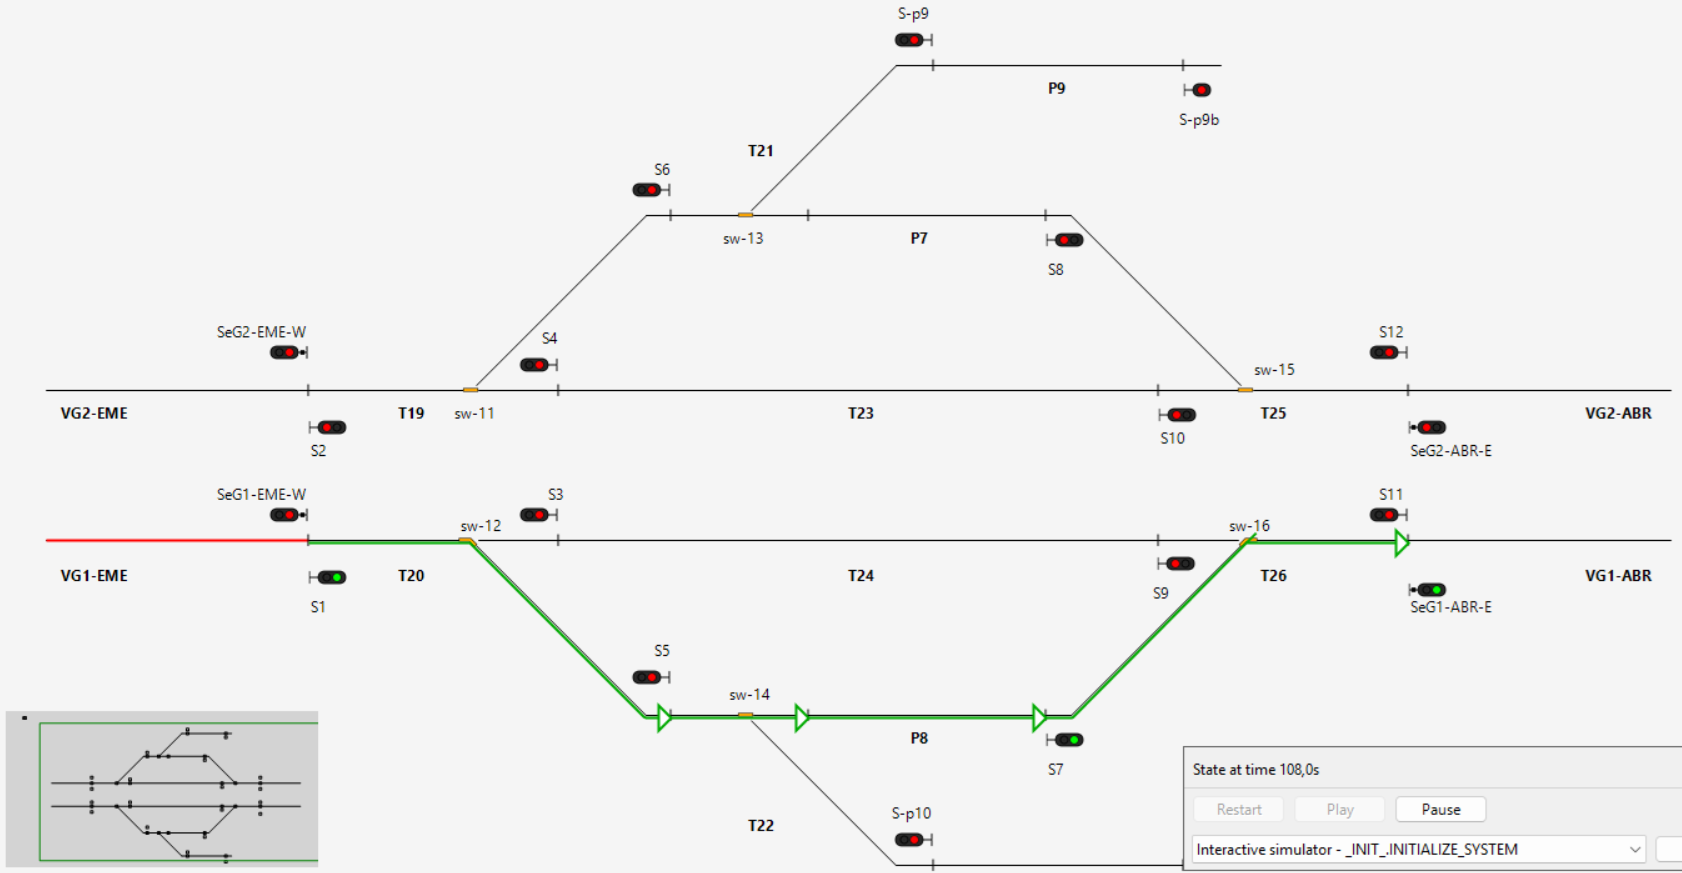
\includegraphics[width=0.92\linewidth,height=4.8cm,keepaspectratio]{../img/simulation_1.png}\par
  \vspace*{1.5mm}
  \begin{proverbox}{Engineering Observations at t = 108.0s}
    \fontsize{6.2}{7.4}\selectfont
    Train dispatched from \texttt{VG1-EME} into platform track \texttt{P8}. Route locks successfully; point machines \texttt{sw-12} and \texttt{sw-14} detected in reverse/normal correspondence. Siding track \texttt{P10} is safeguarded by flank protection with signal \texttt{S-p10} held at stop.
  \end{proverbox}
\end{frame}

% -----------------------------------------------------------------------------
% BACKUP SLIDE 2: SIMULATION CAPTURE 2 - BOUNDARY HANDOVER
% -----------------------------------------------------------------------------
\begin{frame}{Backup: Simulation Step 2 - Boundary Clearance}{Exit signal S11 clearance into line block VG1-ABR at time t = 160.6s}
  \centering
  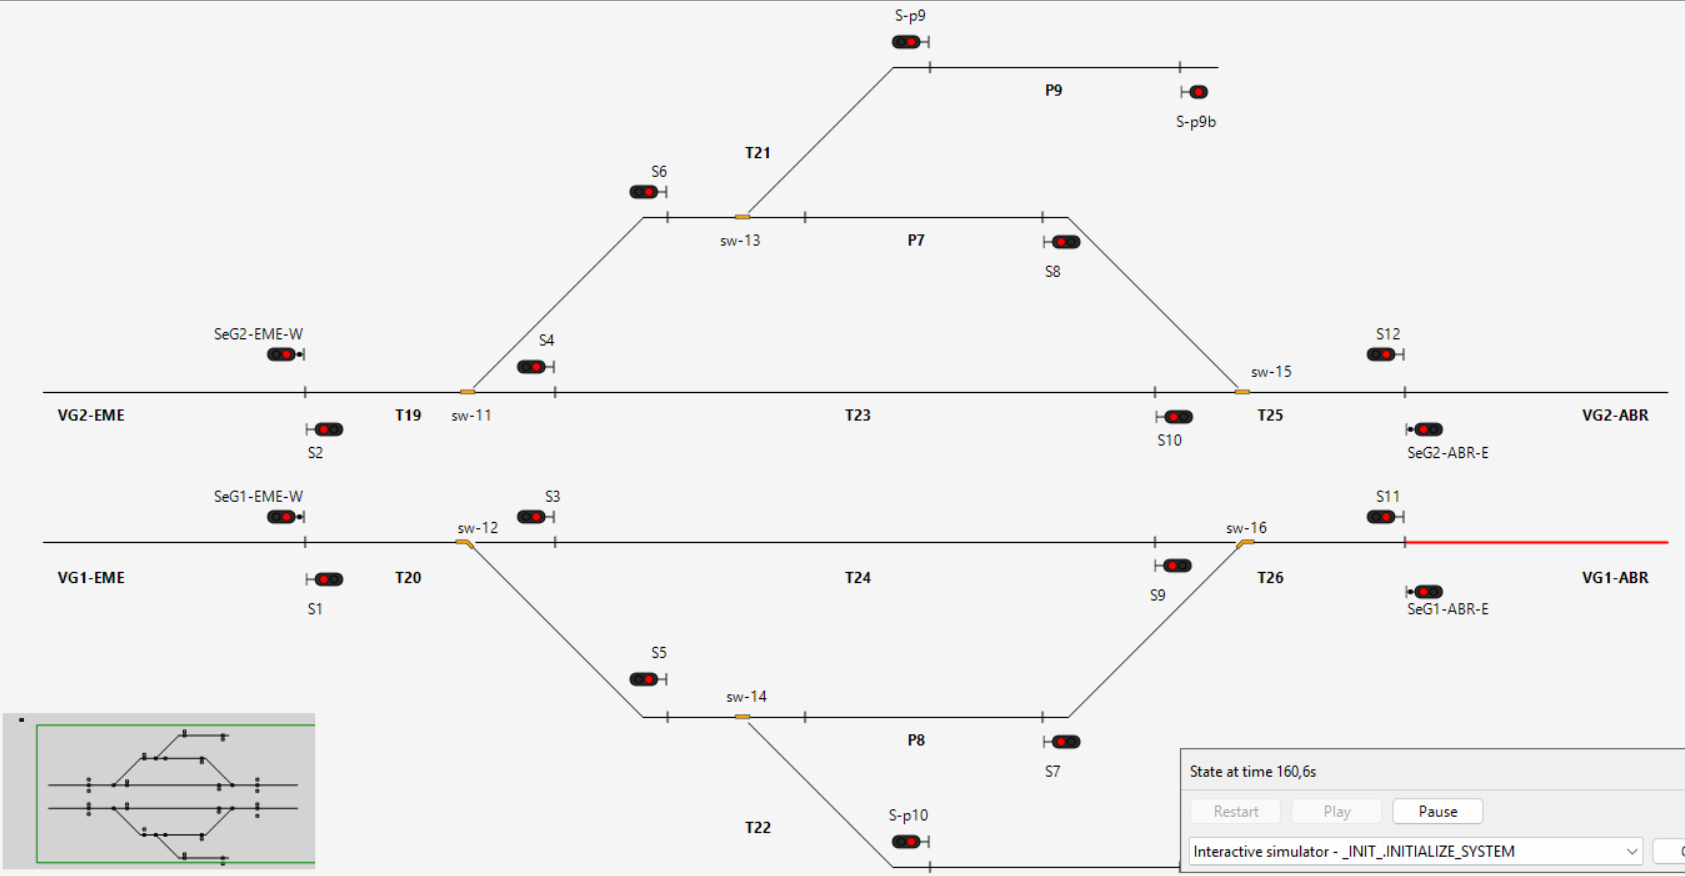
\includegraphics[width=0.92\linewidth,height=4.8cm,keepaspectratio]{../img/simulation_2.png}\par
  \vspace*{1.5mm}
  \begin{proverbox}{Engineering Observations at t = 160.6s}
    \fontsize{6.2}{7.4}\selectfont
    Exit signal \texttt{S11} commands proceed upon receiving \texttt{LineInput=true} from downstream station Clarke over MQTT. As the train advances into line block \texttt{VG1-ABR}, upstream platform route sections sequentially unlock, releasing locks on track \texttt{P8} and switches \texttt{sw-14} and \texttt{sw-16}.
  \end{proverbox}
\end{frame}

% -----------------------------------------------------------------------------
% BACKUP SLIDE 3: SIMULATION CAPTURE 3 - CLARKE ARRIVAL & CROSSOVER
% -----------------------------------------------------------------------------
\begin{frame}{Backup: Simulation Step 3 - Arrival at Clarke}{Scissors crossover transit sw-18 and sw-19 to platform track at time t = 320.4s}
  \centering
  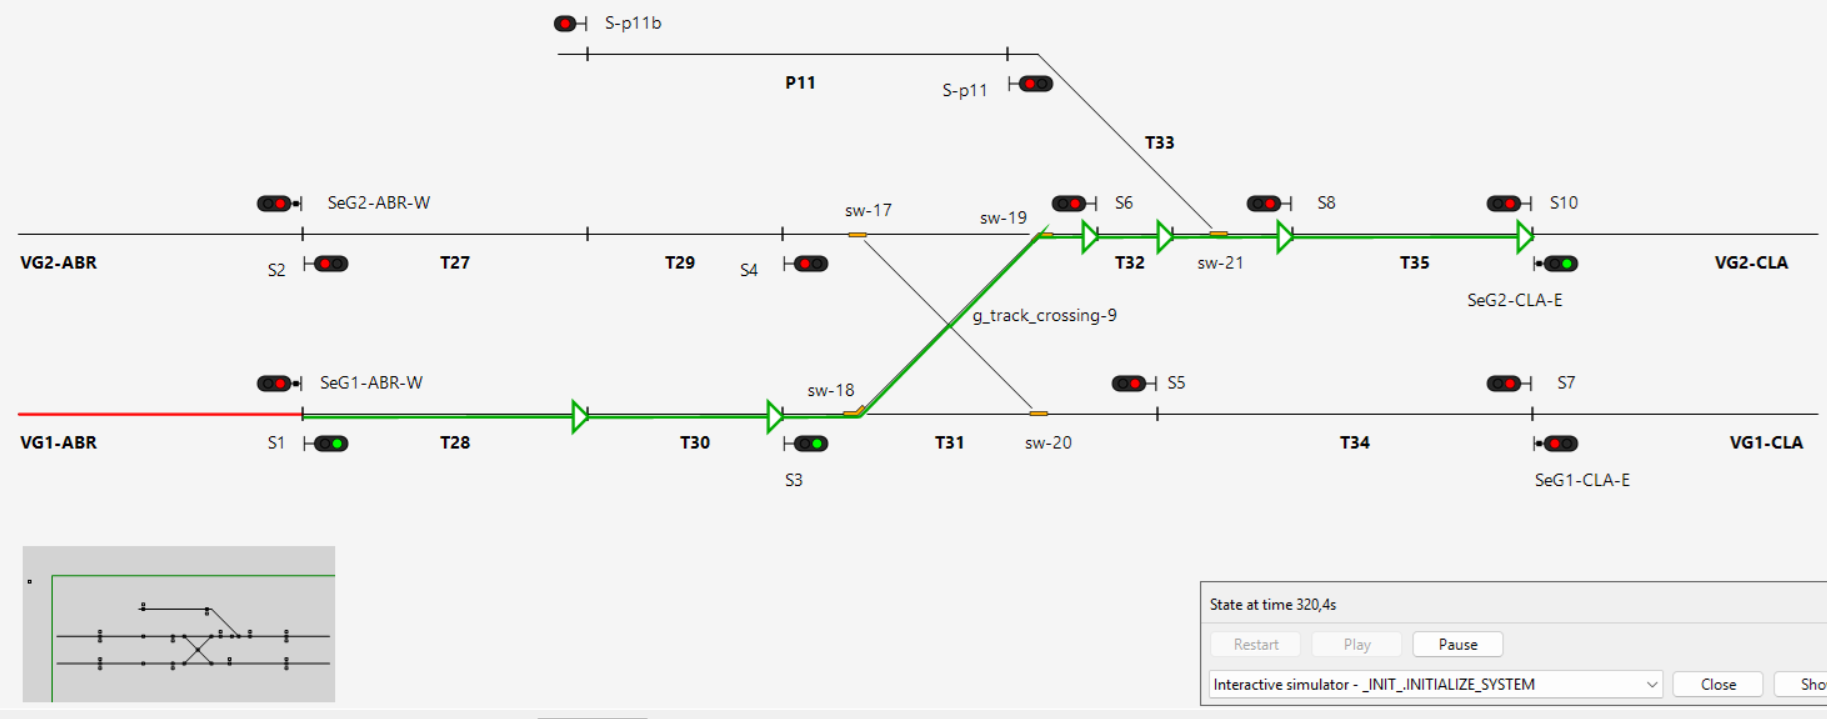
\includegraphics[width=0.92\linewidth,height=4.8cm,keepaspectratio]{../img/simulation_3.png}\par
  \vspace*{1.5mm}
  \begin{proverbox}{Engineering Observations at t = 320.4s}
    \fontsize{6.2}{7.4}\selectfont
    Train arrives at Clarke interlocking area from line track \texttt{VG1-ABR}. Traverses scissors crossover with switches \texttt{sw-18} and \texttt{sw-19} locked in reverse position, establishing guaranteed non-conflicting route to platform track \texttt{T35} under absolute signal protection.
  \end{proverbox}
\end{frame}

% -----------------------------------------------------------------------------
% BACKUP SLIDE 4: TEMPORAL SEMANTICS OF GSS_10
% -----------------------------------------------------------------------------
\begin{frame}{Backup: Temporal Semantics of GSS 10}{Cycle evaluation and temporal formalization with the PRE operator}
  \begin{columns}[c]
    \begin{column}{0.50\textwidth}
      \begin{proverbox}{Requirement 10 Mathematical Definition}
        \fontsize{6.2}{7.4}\selectfont
        \begin{equation*}
          \begin{aligned}
            & \mathbf{PRE}\,\texttt{Locked}(rts) \land \sim\texttt{Locked}(rts) \\
            & \land \sim\mathbf{SOME}\,rt \Big(\texttt{route\_sections}(rt, rts) \land rt.\texttt{JustUnlocked} \\
            & \quad \land \sim rt.\texttt{immediate\_manual\_release} \\
            & \quad \land \sim\mathbf{SOME}\,rt1 (\sim(rt1 = rt) \land \texttt{route\_sections}(rt1, rts) \\
            & \qquad \land \mathbf{PRE}\,rt1.\texttt{Holding} \land \sim rt1.\texttt{JustUnlocked})\Big) \\
            & \implies \mathbf{ALL}\,tc (\texttt{tracks}(rts, tc) \implies \texttt{Clear}(tc)) \\
            & \quad \land \mathbf{PRE}\,\texttt{ready\_to\_release}(rts)
          \end{aligned}
        \end{equation*}
      \end{proverbox}
    \end{column}

    \begin{column}{0.48\textwidth}
      \begin{proverbox}{Why the \texttt{PRE} Operator is Crucial}
        \begin{itemize}\setlength{\itemsep}{1.5pt}\fontsize{6.5}{7.6}\selectfont
          \item In cycle $t-1$, the train occupies the route section, making \texttt{ready\_to\_release} true.
          \item In cycle $t$, the train moves off the track into the next section; the route section drops its \texttt{Locked} state.
          \item Checking \texttt{ready\_to\_release} in cycle $t$ would evaluate to false because the section is now vacant.
          \item The \textbf{\texttt{PRE}} operator bridges this discrete temporal gap, ensuring formal soundness.
        \end{itemize}
      \end{proverbox}
    \end{column}
  \end{columns}
\end{frame}

% -----------------------------------------------------------------------------
% BACKUP SLIDE 5: MANUAL ROUTE RELEASE STATE MACHINE
% -----------------------------------------------------------------------------
\begin{frame}{Backup: Manual Route Release Transitions}{State machine behavior and overlapping route holding protection}
  \begin{columns}[c]
    \begin{column}{0.48\textwidth}
      \begin{proverbox}{Route Release State Machine}
        \centering\vspace{1mm}
        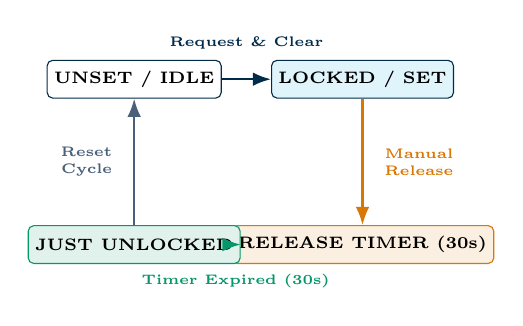
\begin{tikzpicture}[
          x=1cm, y=1cm,
          state/.style={draw=ProverNavy, fill=white, rounded corners=2pt, font=\fontsize{6.2}{7.2}\selectfont\bfseries, inner sep=2.5pt, minimum width=1.85cm, minimum height=0.48cm, align=center}
        ]
          % 4 States in clean clockwise rectangle
          \node[state] (idle) at (0.2, 2.6) {UNSET / IDLE};
          \node[state, fill=ProverTeal!12] (locked) at (3.1, 2.6) {LOCKED / SET};
          \node[state, draw=MetroOrange, fill=MetroOrange!12, minimum width=2.1cm] (timer) at (3.1, 0.5) {RELEASE TIMER (30s)};
          \node[state, draw=SafeGreen, fill=SafeGreen!12] (unlocked) at (0.2, 0.5) {JUST UNLOCKED};

          % Transitions with spacious, non-overlapping labels
          \draw[->, >=Latex, thick, ProverNavy] (idle) -- (locked)
            node[midway, above=2.5mm, font=\fontsize{5.2}{6.2}\selectfont\bfseries\color{ProverNavy}] {Request \& Clear};

          \draw[->, >=Latex, thick, MetroOrange] (locked) -- (timer)
            node[midway, right=1.5mm, font=\fontsize{5.2}{6.2}\selectfont\bfseries\color{MetroOrange}, align=left] {Manual\\Release};

          \draw[->, >=Latex, thick, SafeGreen] (timer) -- (unlocked)
            node[midway, below=2.5mm, font=\fontsize{5.2}{6.2}\selectfont\bfseries\color{SafeGreen!90!black}] {Timer Expired (30s)};

          \draw[->, >=Latex, thick, ProverSlate] (unlocked) -- (idle)
            node[midway, left=1.5mm, font=\fontsize{5.2}{6.2}\selectfont\bfseries\color{ProverSlate}, align=right] {Reset\\Cycle};
        \end{tikzpicture}
      \end{proverbox}
    \end{column}

    \begin{column}{0.50\textwidth}
      \begin{proverbox}{Concurrency and Overlap Resolution}
        \begin{itemize}\setlength{\itemsep}{1.5pt}\fontsize{6.5}{7.6}\selectfont
          \item \textbf{Scenario:} Route $A$ and Route $B$ share route section $S_1$.
          \item Route $A$ is locked. Dispatcher initiates manual release on Route $A$.
          \item If Route $B$ requests lock during the countdown:
            \begin{itemize}\fontsize{6}{7}\selectfont
              \item \texttt{Holding} latch on Route $A$ remains active.
              \item $S_1$ is barred from releasing under Route $B$.
              \item Once Route $A$'s timer expires, $S_1$ transitions safely to Route $B$ without any transient hazard.
            \end{itemize}
        \end{itemize}
      \end{proverbox}
    \end{column}
  \end{columns}
\end{frame}

% -----------------------------------------------------------------------------
% BACKUP SLIDE 6: EXIT SIGNAL & LINE BLOCK PROTOCOL
% -----------------------------------------------------------------------------
\begin{frame}{Backup: Line Block Handshake Protocol}{Sequential interface signals between adjacent interlocking stations}
  \begin{columns}[c]
    \begin{column}{0.50\textwidth}
      \begin{proverbox}{Handshake Sequence Between Station A and Station B}
        \fontsize{6.2}{7.4}\selectfont
        \begin{enumerate}\setlength{\itemsep}{1.2pt}
          \item \textbf{Quiescent State:} Neither station has a locked route to line track \texttt{VG1}. Both output $\texttt{LineOutput} = \texttt{true}$.
          \item \textbf{Dispatch Request at A:} Route locked to \texttt{SeG1-A-E}. Station A asserts internal \texttt{end\_locked}.
          \item \textbf{Clearance Evaluation:}
            \begin{equation*}
              \begin{aligned}
                \texttt{CommandedProceed} \iff & \texttt{end\_locked} \land \text{LineInput}_A \\
                & \land \texttt{Clear}(VG1)
              \end{aligned}
            \end{equation*}
          \item \textbf{Line Reservation:} Station A asserts proceed on \texttt{SeG1-A-E} $\implies$ $\text{LineOutput}_A$ drops to \texttt{false}.
          \item \textbf{Boundary Lockout at B:} Station B detects $\sim\text{LineInput}_B$ $\implies$ opposite entry strictly forbidden.
        \end{enumerate}
      \end{proverbox}
    \end{column}

    \begin{column}{0.48\textwidth}
      \begin{proverbox}{Requirements EXIT 1 and EXIT 2 Summary}
        \fontsize{6.5}{7.6}\selectfont
        \begin{itemize}\setlength{\itemsep}{1.5pt}
          \item \textbf{\texttt{EXIT\_1}:} \texttt{LineOutput} is true only when unreserved, uncommanded to proceed and line track clear.
          \item \textbf{\texttt{EXIT\_2}:} Exit signal commanded to proceed only when end-locked, line input is true and line track is vacant.
        \end{itemize}
      \end{proverbox}

      \begin{safebox}{Safety Assurance}
        \fontsize{6.5}{7.6}\selectfont
        Guarantees head-on collision impossibility between adjacent stations.
      \end{safebox}
    \end{column}
  \end{columns}
\end{frame}

% -----------------------------------------------------------------------------
% BACKUP SLIDE 7: VERIFICATION METRICS & COMPLEXITY ANALYSIS
% -----------------------------------------------------------------------------
\begin{frame}{Backup: Solver Performance Metrics}{Induction depth and verification execution time across stations}
  \begin{columns}[c]
    \begin{column}{0.65\textwidth}
      \begin{proverbox}{Detailed Station Complexity and Model Checking Metrics}
        \fontsize{6.2}{7.4}\selectfont
        \begin{tabularx}{\linewidth}{Xccccc}
          \toprule
          \textbf{Metric} & \textbf{G-PEX} & \textbf{G-EME} & \textbf{G-ABR} & \textbf{G-CLA} & \textbf{G-TEC} \\
          \midrule
          \textbf{Switches} & 5 & 5 & 6 & 5 & 5 \\
          \textbf{Signals} & 15 & 18 & 20 & 15 & 22 \\
          \textbf{Tracks} & 11 & 11 & 10 & 11 & 11 \\
          \textbf{Routes} & 14 & 16 & 22 & 16 & 20 \\
          \textbf{Max $k$} & 1 & 1 & 1 & 1 & 1 \\
          \textbf{Time} & 12.4\,s & 14.8\,s & 19.2\,s & 13.6\,s & 18.5\,s \\
          \textbf{Status} & \color{SafeGreen}\textbf{PROVED} & \color{SafeGreen}\textbf{PROVED} & \color{SafeGreen}\textbf{PROVED} & \color{SafeGreen}\textbf{PROVED} & \color{SafeGreen}\textbf{PROVED} \\
          \bottomrule
        \end{tabularx}
      \end{proverbox}
    \end{column}

    \begin{column}{0.33\textwidth}
      \begin{proverbox}{Inductive Invariant Power}
        \begin{itemize}\setlength{\itemsep}{1.5pt}\fontsize{6.5}{7.6}\selectfont
          \item All 60 goals were proven via \textbf{1-step induction} ($k=1$), confirming the invariant inductivity of the system design.
          \item No auxiliary induction lemmas needed to be hand-crafted, validating the architectural elegance of the GDS.
        \end{itemize}
      \end{proverbox}
    \end{column}
  \end{columns}
\end{frame}

\end{document}
